\documentclass[aspectratio=169,11pt,t]{beamer}
% ============================================================
%  ksa-cs-v2: ksa-cs-lecture-template.tex 스타일 + 한글, v2 덱(16:9)용.
%    - 짙은 네이비 헤드라인 (섹션 이름 + 프레임마다 점)
%    - 꽉 찬 파란 제목 막대, 둥근 그림자 블록
%    - 한글: Noto Sans CJK KR (fontspec)
%  사용:
%    \documentclass[aspectratio=169,11pt,t]{beamer}
%    \input{<..>/theme/ksa-cs-v2.tex}
%  ksa-theme.tex 의 매크로(\kb \kq, ksablue/ksared 등)도 같은 이름으로 둔다
%  -> v2 덱 본문을 거의 그대로 옮길 수 있다.
% ============================================================

\usepackage{fontspec}
\usepackage{amsmath,amssymb}
\usepackage{tikz}
\usepackage{listings}
\usepackage{graphicx}
\usepackage{booktabs}
\usepackage{varwidth}
% enumitem 은 넣지 않는다 (beamer 글머리표가 사라진다)

\defaultfontfeatures{Ligatures=TeX}
\setmainfont{Noto Sans CJK KR}
\setsansfont{Noto Sans CJK KR}
\setmonofont{Noto Sans Mono CJK KR}[Scale=0.92]
\usefonttheme{professionalfonts}

% ---------- 기본 틀 ----------
\usetheme{default}
\useinnertheme[shadow=true]{rounded}
\setbeamertemplate{navigation symbols}{}
\setbeamersize{text margin left=1em,text margin right=1em}

% ---------- 색 (템플릿 원본 값) ----------
\definecolor{navydark}{HTML}{191959}
\definecolor{navydim}{HTML}{8888B0}
\definecolor{navytitle}{HTML}{262686}
\definecolor{navyblue}{HTML}{3333B2}
\definecolor{blockbodybg}{HTML}{E9E9F3}
\definecolor{examplegreen}{HTML}{006000}
\definecolor{examplebg}{HTML}{E5EFE5}
\definecolor{alertred}{HTML}{BF0000}
\definecolor{alertbg}{HTML}{F9E5E5}
% ksa-theme.tex 와 같은 이름 (본문 호환)
\colorlet{ksablue}{navytitle}
\colorlet{ksabluedk}{navydark}
\definecolor{ksagold}{HTML}{D6CBB1}
\definecolor{ksagolddk}{HTML}{A9976B}
\colorlet{ksared}{alertred}
\definecolor{ksagray}{HTML}{5B5B5B}

\setbeamercolor{structure}{fg=navyblue}
\setbeamercolor{alerted text}{fg=alertred}
\setbeamercolor{frametitle}{bg=navytitle,fg=white}
\setbeamercolor{title}{fg=white,bg=navytitle}
\setbeamercolor{block title}{bg=navytitle,fg=white}
\setbeamercolor{block body}{bg=blockbodybg,fg=black}
\setbeamercolor{block title example}{bg=examplegreen,fg=white}
\setbeamercolor{block body example}{bg=examplebg,fg=black}
\setbeamercolor{block title alerted}{bg=alertred,fg=white}
\setbeamercolor{block body alerted}{bg=alertbg,fg=black}
\setbeamercolor{item}{fg=navyblue}
\setbeamertemplate{itemize item}[circle]
\setbeamertemplate{itemize subitem}[triangle]

% ---------- 헤드라인: miniframes (섹션 이름 + 점) ----------
\useoutertheme[subsection=false]{miniframes}
\setbeamerfont{section in head/foot}{size=\tiny}
\setbeamercolor{section in head/foot}{bg=navydark,fg=white}
\setbeamercolor{mini frame}{fg=white}
\setbeamertemplate{mini frames}[circle]

% ---------- 제목 막대: 폭 꽉 채움, 두 줄까지 ----------
\setbeamerfont{frametitle}{size=\normalsize,series=\bfseries}
\setbeamertemplate{frametitle}{%
  \nointerlineskip
  \begin{beamercolorbox}[wd=\paperwidth,ht=2.7ex,dp=1.1ex,leftskip=.3cm,rightskip=.3cm]{frametitle}%
    \usebeamerfont{frametitle}\insertframetitle
  \end{beamercolorbox}}

% ---------- 쪽 번호: 오른쪽 아래 ----------
\setbeamertemplate{footline}{%
  \hfill
  {\color{navydim}\scriptsize\insertframenumber\,/\,\inserttotalframenumber}%
  \hspace{3mm}\vspace{2mm}%
}

% ---------- 표지: 템플릿처럼 헤드라인은 그대로, 가운데 둥근 그림자 상자에 제목 한 줄 ----------
% 덱에서:  {\setbeamertemplate{footline}{}\begin{frame}[c,noframenumbering]\titlepage\end{frame}}
\setbeamercolor{title}{fg=white,bg=navyblue}
\makeatletter
\setbeamertemplate{title page}{%
  \vfill
  \centering
  \begin{minipage}{0.84\paperwidth}
  \begin{beamercolorbox}[wd=\linewidth,sep=7pt,center,rounded=true,shadow=true]{title}
    {\usebeamerfont{title}\inserttitle\par}%
    \ifx\insertsubtitle\@empty\else\vskip0.4em{\usebeamerfont{subtitle}\insertsubtitle\par}\fi
  \end{beamercolorbox}
  \end{minipage}\par\vskip1.6em
  {\usebeamerfont{author}\color{navytitle}\insertauthor\par}\vskip0.3em
  {\usebeamerfont{institute}\color{ksagray}\insertinstitute\par}
  \vfill
}
\makeatother
\setbeamerfont{title}{series=\bfseries,size=\Large}
\setbeamerfont{subtitle}{size=\normalsize}
\setbeamerfont{author}{size=\normalsize}
\setbeamerfont{institute}{size=\small}

% ksa-theme 호환: 덱이 \renewcommand{\ksacredit}{..} 를 해도 되게 (꼬리말에는 안 쓴다)
\newcommand{\ksacredit}{}

% ---------- 강조 ----------
\newcommand{\hl}[1]{\textcolor{alertred}{#1}}
\newcommand{\hlb}[1]{\textcolor{navyblue}{#1}}
\newcommand{\kb}[1]{\textbf{\color{ksablue}#1}}
\newcommand{\kq}[1]{\textbf{\color{ksared}#1}}

% ---------- 파이썬 코드 (템플릿과 같은 색) ----------
\definecolor{codekw}{HTML}{0033B3}
\definecolor{codebuiltin}{HTML}{BF0000}
\definecolor{codestr}{HTML}{067D17}
\definecolor{codecomment}{HTML}{8C8C8C}
\definecolor{codenum}{HTML}{1750EB}
\lstdefinestyle{py}{
  language=Python, basicstyle=\ttfamily\scriptsize,
  keywordstyle=\color{codekw}\bfseries, stringstyle=\color{codestr},
  commentstyle=\color{codecomment}\itshape, numberstyle=\color{codenum},
  emph={print,len,range,sum,input,int,str,float,list,dict,append,remove,sorted,abs,min,max},
  emphstyle=\color{codebuiltin}, showstringspaces=false, keepspaces=true,
  columns=fixed, basewidth=0.52em, aboveskip=1mm, belowskip=1mm, xleftmargin=2mm,
  breaklines=true
}
\lstset{style=py}

% 원본 덱 (ksa-theme): slides/v2/ml1/week09/vanishing_gradient/ -- 그림은 거기 figs/ 를 그대로 쓴다
\setbeamerfont{author}{size=\normalsize}
\setbeamerfont{institute}{size=\small}
\graphicspath{{../../../v2/ml1/week09/vanishing_gradient/figs/}{../../../assets/}}
\makeatletter
\newcommand{\markpage}[1]{\protected@write\@auxout{}{\string\newlabel{#1}{{\the\c@framenumber}{}}}\hypertarget{#1}{}}
\newcommand{\pref}[1]{\hyperlink{#1}{\textcolor{ksagolddk}{(p.\ref{#1})}}}
\makeatother

\renewcommand{\ksacredit}{Machine Learning and Deep Learning \,\textperiodcentered\, 기울기 소실}
\title{기울기 소실 (Vanishing Gradient)}
\subtitle{층을 쌓을수록 학습이 멈춘다? 활성 함수와 초기화}
\author{Machine Learning and Deep Learning}
\institute{한국과학영재학교 (KSA)}
\date{}
\begin{document}
{\setbeamertemplate{footline}{}\begin{frame}[c,noframenumbering]\titlepage\end{frame}}

\section{질문}
% --- 오늘의 질문
\begin{frame}{오늘의 질문}
\vfill
\centering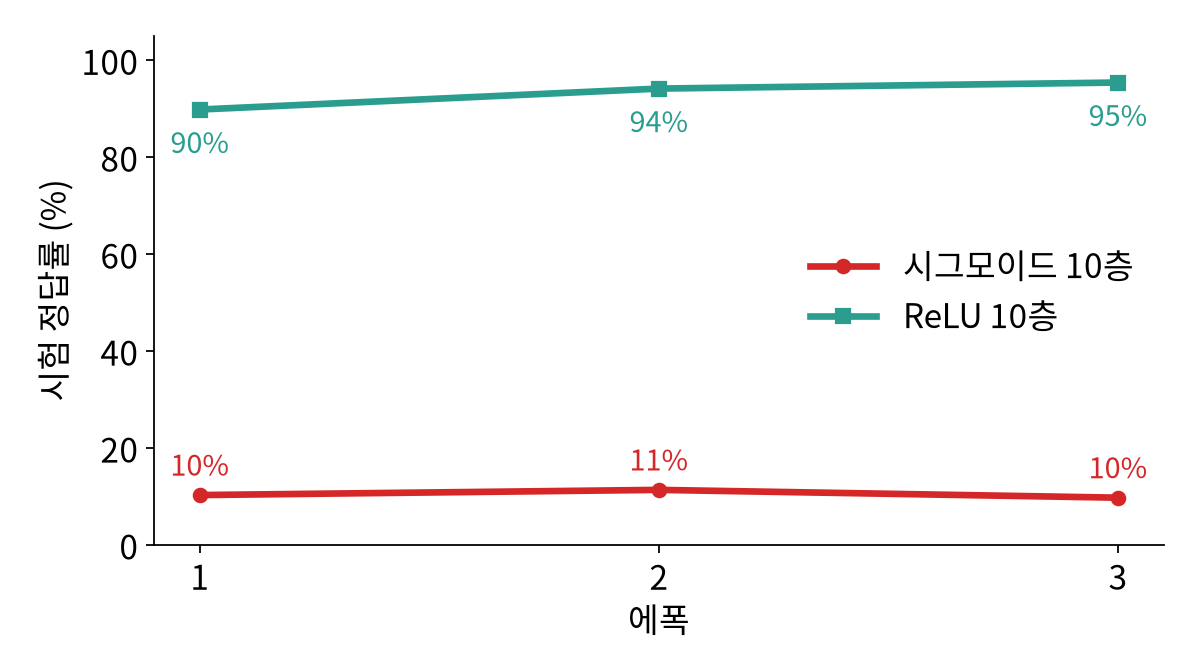
\includegraphics[width=0.56\linewidth]{vg_acc.png}\par\vskip0.2em
{\large MNIST, 은닉층 \textbf{10개}, 활성 함수만 다르다: \kq{시그모이드 10\% vs ReLU 95\%}}
\vfill
\note{앞에서 역전파로 XOR을 풀었습니다. 층을 더 깊이 쌓으면 더 어려운 문제도 풀 수 있을 것 같습니다. 그래서 손글씨 숫자 MNIST에 은닉층 10개짜리 신경망을 만들었습니다. 두 신경망은 활성 함수만 다릅니다. 시그모이드를 쓴 쪽은 3에폭이 지나도 정답률 10퍼센트, 열 개 숫자 중 찍는 수준입니다. ReLU를 쓴 쪽은 95퍼센트입니다. 시그모이드 쪽은 학습이 거의 멈춰 있습니다. 왜 그럴까요?}
\end{frame}

\section{소실}
% --- 역전파 복습
\begin{frame}{역전파는 층을 지날 때마다 곱한다}
\vfill
\centering
{\large 역전파 시간 \quad $\delta_1 = \delta_2\,w_2\,\sigma'(z_1)$ \quad (숨은 층 하나)}\vskip0.6em
{\LARGE\[ \delta_{\text{1층}} = \delta_{\text{출구}} \times w_{10}\,\sigma'(z_{9}) \times w_{9}\,\sigma'(z_8) \times \cdots \times w_2\,\sigma'(z_1) \]}\vskip0.4em
{\large 층이 10개면 \textbf{곱하기 10번} \quad 곱하는 수가 1 보다 작으면 \kq{0 으로}, 크면 \kq{폭발}}
\vfill
\note{역전파 시간에 숨은 층의 오차 신호는 출력의 오차 신호에 가중치와 시그모이드 기울기를 곱한 것이었습니다. 층이 10개면 출구에서 입구까지 오는 동안 이 곱셈을 10번 반복합니다. 매번 곱하는 수가 1보다 조금만 작아도 10번 곱하면 0에 가까워지고, 1보다 조금만 커도 폭발합니다. 깊은 신경망의 문제는 이 곱셈에서 나옵니다.}
\end{frame}

% --- 시그모이드 기울기
\begin{frame}{시그모이드의 기울기는 아무리 커도 0.25}
\markpage{sig}
\vfill
\centering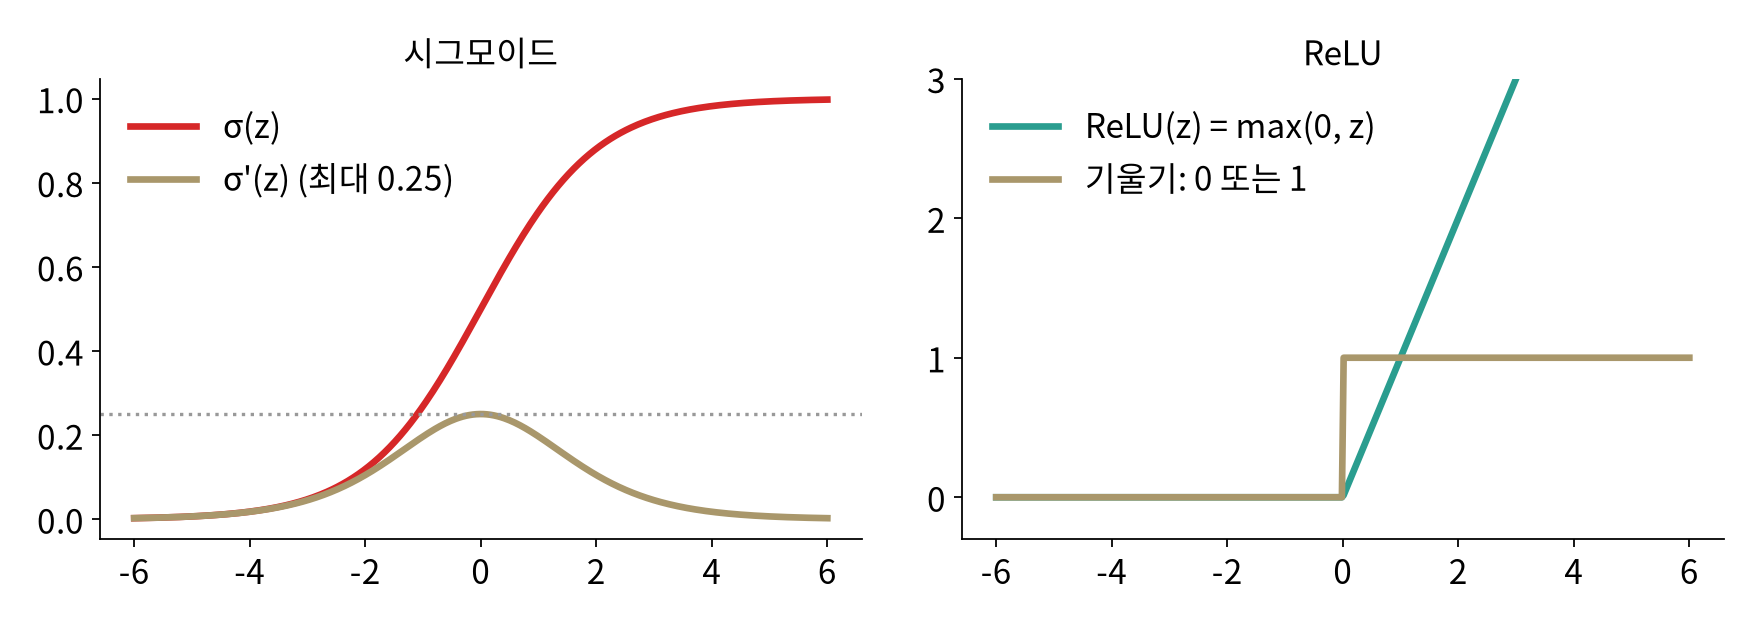
\includegraphics[width=0.80\linewidth]{vg_act.png}\par\vskip0.2em
{\LARGE\[ \sigma'(z) = \sigma(z)\big(1 - \sigma(z)\big) \le 0.25 \qquad 0.25^{10} \approx \kq{0.00000095} \]}
\vfill
\note{시그모이드의 기울기는 시그마 곱하기 1 빼기 시그마입니다. 이 값은 z가 0일 때 0.25로 가장 크고, 양 끝으로 가면 0에 가까워집니다. 그러니 가장 운이 좋아도 층마다 0.25 이하를 곱합니다. 10층이면 0.25의 10제곱, 약 0.00000095, 백만분의 1입니다. 출구의 오차 신호가 입구에 도착할 때는 거의 사라집니다. 이걸 기울기 소실이라고 합니다. 오른쪽 ReLU는 양수일 때 기울기가 정확히 1이라 곱해도 줄지 않습니다.}
\end{frame}

% --- 실제 층별 기울기
\begin{frame}{실제로 재 보면: 입구는 출구의 119만분의 1}
\vfill
\centering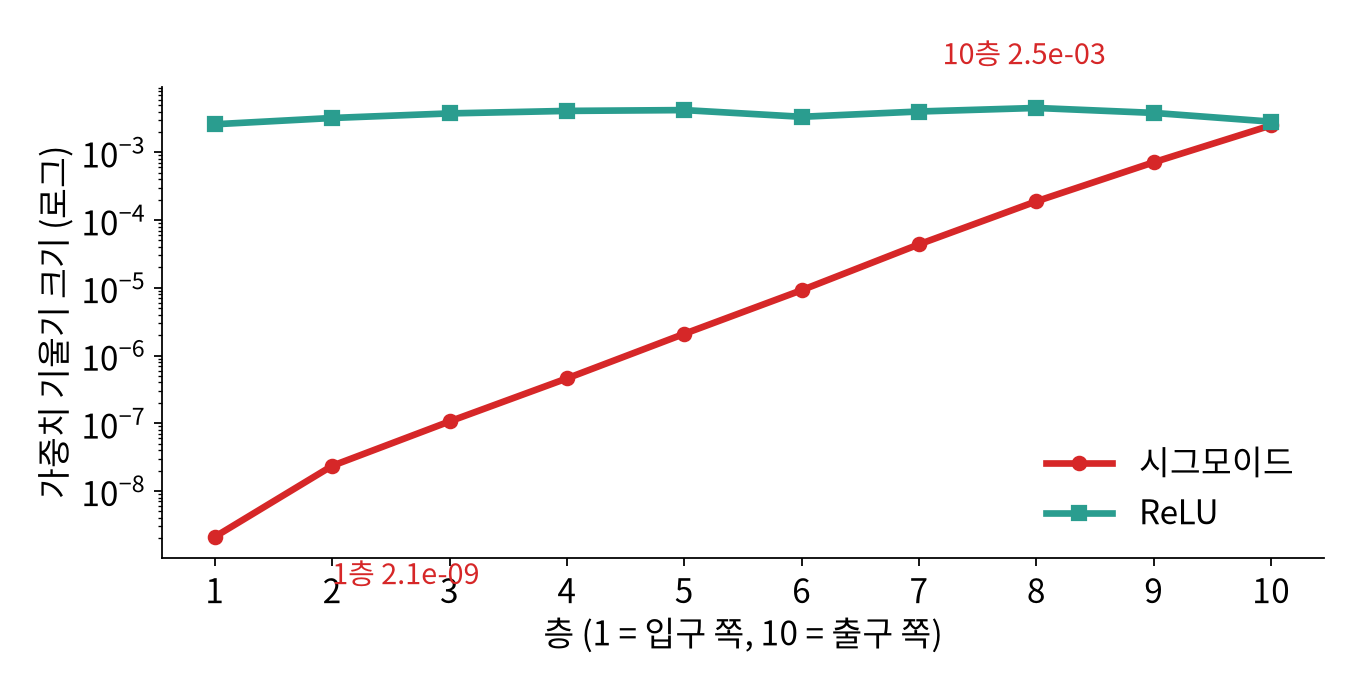
\includegraphics[width=0.6\linewidth]{vg_layers.png}\par\vskip0.2em
{\large 시그모이드: 10층 $2.5 \times 10^{-3}$ $\to$ 1층 $2.1 \times 10^{-9}$ \quad ReLU: 비슷}\\[0.2em]
{\small 학습 전, 배치 512장의 가중치 기울기 평균 절댓값 (Xavier · He 초기화)}
\vfill
\note{실제로 MNIST 신경망에서 층마다 가중치 기울기의 크기를 재 봤습니다. 시그모이드 쪽은 출구인 10층에서 0.0025인데, 입구인 1층에서는 0.0000000021입니다. 119만분의 1입니다. 입구 쪽 층은 학습률을 곱해 가중치를 고쳐도 거의 움직이지 않습니다. 입구가 굳어 있으니 그 뒤의 층들도 쓸모 있는 특징을 받지 못합니다. ReLU 쪽은 1층부터 10층까지 기울기가 비슷한 크기라서 모든 층이 고르게 배웁니다.}
\end{frame}

\section{ReLU}
% --- ReLU
\begin{frame}{해결 1: ReLU}
\vfill
\centering
{\LARGE\[ \text{ReLU}(z) = \max(0, z) \qquad \text{ReLU}'(z) = \begin{cases} 1 & z > 0\\ 0 & z \le 0 \end{cases} \]}\vskip0.4em
{\large 켜진 뉴런은 기울기를 \kb{그대로 (× 1)} 통과시킨다 \quad 계산도 빠르다 (지수 함수 없음)}\\[0.6em]
{\large 같은 10층: \quad 시그모이드 \kq{10\%} \quad $\to$ \quad ReLU \kb{95\%}}\\[0.6em]
{\small 2010년 무렵부터 깊은 신경망의 기본 활성 함수 (AlexNet, 2012)}
\vfill
\note{첫 번째 해결책은 활성 함수를 ReLU로 바꾸는 겁니다. 양수면 그대로, 음수면 0을 냅니다. 기울기는 켜진 뉴런에서 정확히 1이라 곱해도 줄지 않습니다. 지수 함수가 없어 계산도 빠릅니다. 같은 10층 신경망에서 시그모이드 10퍼센트가 ReLU로 95퍼센트가 됐습니다. 2010년 무렵부터 깊은 신경망의 기본 활성 함수가 되었고, 2012년 AlexNet도 ReLU를 썼습니다.}
\end{frame}

\section{폭발 · 초기화}
% --- 폭발
\begin{frame}{반대로: 기울기 폭발}
\vfill
\centering
{\Large 층마다 1.5 를 곱하면 \quad $1.5^{10} \approx \kq{58}$ \qquad 2 를 곱하면 \quad $2^{10} = \kq{1{,}024}$}\\[1.0em]
{\large 기울기가 층마다 커져서 \textbf{한 걸음에 멀리 튀고} 학습이 망가진다 (손실 NaN)}\\[0.8em]
{\large 대책: \textbf{기울기 자르기} (gradient clipping) \quad 크기가 정한 값을 넘으면 줄인다}\\[0.4em]
{\small 순환 신경망 (11주차) 에서 특히 잘 생긴다}
\vfill
\note{반대 문제도 있습니다. 층마다 곱하는 수가 1보다 크면 기울기가 폭발합니다. 1.5를 10번 곱하면 약 58, 2를 10번 곱하면 1024입니다. 그러면 경사하강법이 한 걸음에 엄청나게 멀리 튀어서 손실이 무한대나 NaN이 됩니다. 대책으로 기울기 자르기를 씁니다. 기울기의 크기가 정한 값을 넘으면 방향은 그대로 두고 크기만 줄여서 씁니다. 11주차 순환 신경망에서 특히 자주 생깁니다.}
\end{frame}

% --- 초기화
\begin{frame}{해결 2: 가중치 초기화}
\markpage{init}
\vfill
\centering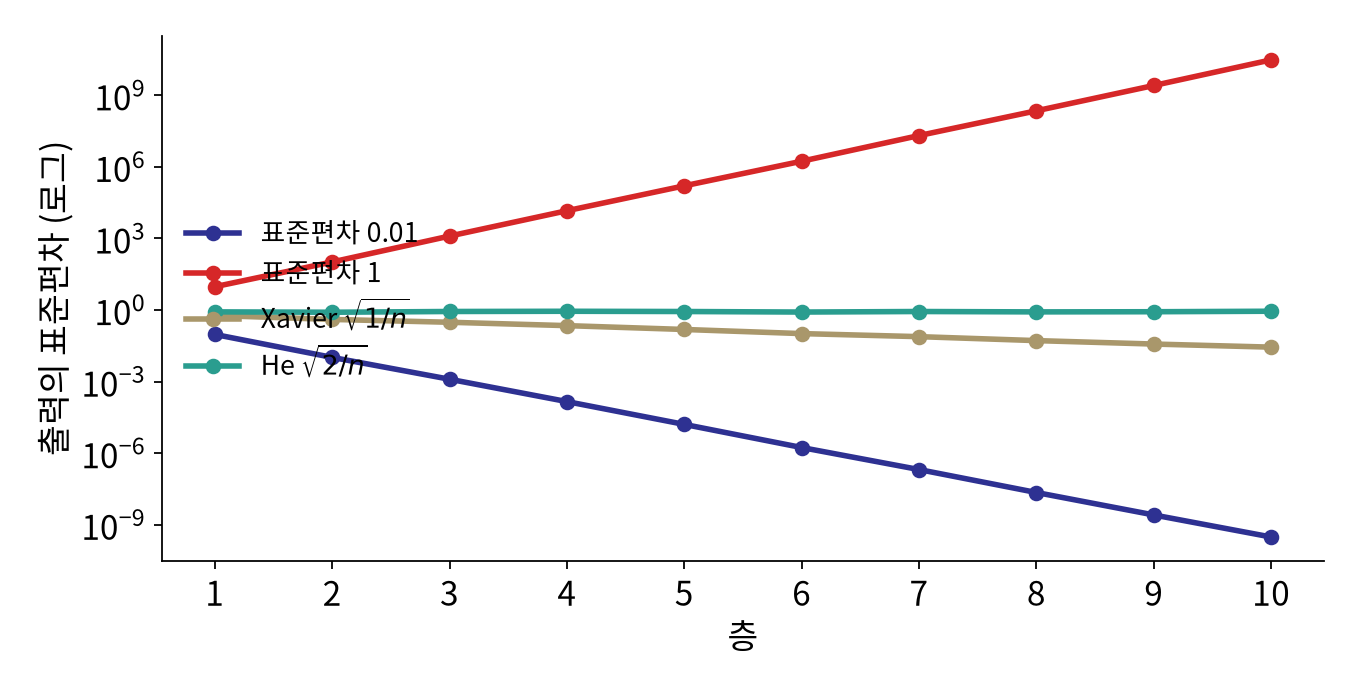
\includegraphics[width=0.58\linewidth]{vg_init.png}\par\vskip0.2em
{\large ReLU 10층, 시작 표준편차만 바꿈: \; 0.01 $\to$ \kq{$3 \times 10^{-10}$} \; 1 $\to$ \kq{$3 \times 10^{10}$} \; He $\to$ \kb{0.88}}
\vfill
\note{두 번째 해결책은 가중치를 처음에 어떤 크기로 놓느냐입니다. 순전파에서도 같은 곱셈 문제가 생깁니다. ReLU 10층 신경망에 무작위 입력을 넣고, 시작 가중치의 표준편차만 바꿔 층별 출력의 크기를 쟀습니다. 0.01로 작게 시작하면 층마다 줄어들어 10층에서 10의 마이너스 10제곱, 사라집니다. 1로 크게 시작하면 10의 10제곱으로 폭발합니다. 초록 He 초기화는 10층까지 0.8에서 1 사이로 일정합니다. 노란 Xavier 초기화는 ReLU에서는 조금씩 줄어듭니다.}
\end{frame}

% --- Xavier He
\begin{frame}{크기를 층마다 유지하는 초기화}
\vfill
\centering
{\large 입력 $n$ 개를 받는 뉴런: 가중치 $n$ 개의 곱의 합 \quad $\to$ 분산이 $n \times \text{Var}(w)$ 배로}\vskip0.6em
\renewcommand{\arraystretch}{1.5}
{\large\begin{tabular}{lll}
\textbf{Xavier} (Glorot, 2010) & $\text{Var}(w) = \dfrac{1}{n}$ & 시그모이드 · tanh\\
\textbf{He} (2015) & $\text{Var}(w) = \dfrac{2}{n}$ & \kb{ReLU} (절반을 0 으로 버리니 2배)
\end{tabular}}\vskip0.6em
{\small PyTorch \texttt{nn.Linear} 의 기본값도 이런 크기 조정을 한다 \quad 폭 256 이면 He 의 표준편차 $\sqrt{2/256} \approx 0.088$}
\vfill
\note{어떻게 정할까요? 뉴런 하나는 입력 n개에 가중치를 곱해 더합니다. 입력과 가중치가 독립이면 출력의 분산은 대략 n 곱하기 가중치의 분산 배가 됩니다. 이게 1이 되도록 가중치의 분산을 n분의 1로 두는 것이 Xavier 초기화입니다. ReLU는 음수 절반을 0으로 버려 분산이 절반으로 줄기 때문에 2배인 n분의 2로 둡니다. 이것이 He 초기화입니다. 폭이 256이면 표준편차는 약 0.088입니다. PyTorch의 Linear 층도 기본으로 이런 크기 조정을 해 줍니다.}
\end{frame}

% --- ReLU 단점
\begin{frame}{ReLU 의 약점과 친척들}
\vfill
\centering
\renewcommand{\arraystretch}{1.5}
{\large\begin{tabular}{ll}
\kq{죽은 ReLU} & 늘 음수만 받는 뉴런은 기울기가 항상 0 $\to$ 영영 안 배운다\\
\textbf{Leaky ReLU} & 음수 쪽에 작은 기울기 ($0.01z$) 를 남긴다\\
\textbf{GELU} & 매끄러운 ReLU \quad 트랜스포머 (GPT · BERT) 의 기본
\end{tabular}}\vskip0.8em
{\large 그 밖에: \textbf{배치 정규화} (다음 시간), \textbf{잔차 연결} (9주차), \textbf{LSTM} (11주차)}
\vfill
\note{ReLU에도 약점이 있습니다. 어떤 뉴런이 학습 중에 늘 음수만 받게 되면 기울기가 항상 0이라 그 뉴런은 영영 다시 배우지 못합니다. 죽은 ReLU라고 부릅니다. 그래서 음수 쪽에 0.01 같은 작은 기울기를 남기는 Leaky ReLU, 매끄럽게 만든 GELU 같은 친척들이 있고, GPT나 BERT 같은 트랜스포머는 GELU를 씁니다. 기울기 소실을 해결하는 방법은 이 밖에도 있습니다. 다음 시간의 배치 정규화, 9주차 ResNet의 잔차 연결, 11주차 LSTM의 문이 모두 같은 문제를 다른 방식으로 푼 것입니다.}
\end{frame}

\section{연습}
% --- 문제풀이
\begin{frame}{문제풀이}
\vfill
\begin{enumerate}
\item 시그모이드 신경망 20층에서, 가장 운이 좋아도 입구의 오차 신호는 출구의 몇 배인가? ($0.25^{10} \approx 10^{-6}$)\vskip0.8em
\item ReLU 뉴런의 입력 $z$ 가 $-3$, $0.5$, $2$ 일 때 출력과 기울기는?\vskip0.8em
\item 입력이 512 개인 ReLU 층의 He 초기화 표준편차는?\vskip0.8em
\item 학습 중 손실이 갑자기 NaN 이 됐다. 의심할 것과 대책 두 가지는?
\end{enumerate}
\vfill
\note{1번 답. 0.25의 20제곱, 0.25의 10제곱의 제곱이니 약 10의 마이너스 12제곱입니다. 2번 답. 마이너스 3은 출력 0, 기울기 0, 0.5는 출력 0.5, 기울기 1, 2는 출력 2, 기울기 1입니다. 3번 답. 루트 512분의 2, 루트 256분의 1, 16분의 1, 0.0625입니다. 4번 답. 기울기 폭발을 의심하고, 학습률을 줄이거나 기울기 자르기를 씁니다. 초기화를 점검하는 것도 좋습니다.}
\end{frame}

% --- 실습
\begin{frame}{실습}
\vfill
\centering\begin{tabular}{rl}
\large 1 & 층마다 곱하기: 시그모이드 기울기 0.25 를 10번, 20번 \quad 초기화별 층 출력 크기\\[0.5em]
\large 2 & PyTorch 10층 신경망 (MNIST): 시그모이드 vs ReLU 의 층별 기울기 재기\\[0.5em]
\large 3 & 같은 신경망을 1에폭 학습해 정답률 비교 + Leaky ReLU · GELU
\end{tabular}\vskip1em
MNIST (LeCun, Cortes, Burges; torchvision) \\[0.4em]\href{https://colab.research.google.com/github/SuminHan/book-ml/blob/main/slides/v2/ml1/week09/vanishing_gradient/lab/vanishing_gradient.ipynb}{\textcolor{ksagolddk}{▶ Colab에서 실습 노트북 열기}}
\vfill
\note{실습은 세 부분입니다. 첫째, 시그모이드 기울기를 층마다 곱해 보고, 초기화에 따라 층 출력의 크기가 어떻게 변하는지 numpy로 재현합니다. 둘째, PyTorch로 10층 신경망을 만들어 MNIST 배치 하나로 층별 기울기 크기를 시그모이드와 ReLU에서 잽니다. 셋째, 같은 신경망을 1에폭 학습해서 정답률을 비교하고, Leaky ReLU와 GELU도 넣어 봅니다.}
\end{frame}

\section{정리}
% --- 정리
\begin{frame}{정리}
\vfill
\centering\large\begin{tabular}{l}
역전파는 층마다 곱한다 \quad 1 보다 작으면 \kq{소실}, 크면 \kq{폭발}\\[0.5em]
시그모이드 기울기 $\le 0.25$ $\to$ 10층에서 입구 기울기 119만분의 1, 정답률 10\%\\[0.5em]
\textbf{ReLU}: 켜진 뉴런은 기울기 1 $\to$ 95\% \quad (죽은 ReLU $\to$ Leaky ReLU, GELU)\\[0.5em]
\textbf{초기화}: Xavier $1/n$, He $2/n$ 로 층마다 크기 유지 \quad 폭발엔 기울기 자르기
\end{tabular}
\vfill
\note{정리합니다. 역전파는 층을 지날 때마다 곱하기 때문에 곱하는 수가 1보다 작으면 기울기가 사라지고, 크면 폭발합니다. 시그모이드의 기울기는 0.25 이하라서 10층에서 입구 기울기가 출구의 119만분의 1이 되고 학습이 멈춥니다. ReLU는 켜진 뉴런의 기울기가 1이라 같은 신경망이 95퍼센트까지 갑니다. 그리고 가중치 초기화를 Xavier나 He 방식으로 하면 층마다 크기가 유지되고, 폭발에는 기울기 자르기를 씁니다.}
\end{frame}
\end{document}
